% Created 2024-11-04 Mon 16:19
% Intended LaTeX compiler: pdflatex
\documentclass[11pt]{article}
\usepackage[utf8]{inputenc}
\usepackage[T1]{fontenc}
\usepackage{graphicx}
\usepackage{longtable}
\usepackage{wrapfig}
\usepackage{rotating}
\usepackage[normalem]{ulem}
\usepackage{amsmath}
\usepackage{amssymb}
\usepackage{capt-of}
\usepackage{hyperref}
\usepackage{amsmath}
\usepackage{cite}
\usepackage{float}
\usepackage[nottoc,numbib]{tocbibind}
\date{\today}
\title{Elektrooptični pojav}
\hypersetup{
 pdfauthor={},
 pdftitle={Elektrooptični pojav},
 pdfkeywords={},
 pdfsubject={},
 pdfcreator={Emacs 29.4 (Org mode 9.7.11)}, 
 pdflang={English}}


\renewcommand{%
  \refname}{Viri}

\title{
  
\includegraphics[width=0.4\textwidth]{fmf_logo}\\
  {\small Oddelek za fiziko} \\
  {Elektrooptični pojav}\\
  {\small Poročilo vaje pri FP5}\\

}
\date{}
\author{ Kristofer Čepon Povšič \\[5 cm]
  \small  Asistent: Tilen Knaflič  \\
}
\newfloat{slika}{htbp}{loc}
\floatname{slika}{Slika}

\newfloat{tabela}{htbp}{loc}
\floatname{tabela}{Tabela}

\begin{document}

\maketitle
\pagebreak
\tableofcontents\pagebreak
\section{Uvod}\label{sec:org38a6132}

Tekoče kristale tvorijo podolgovate molekule, ki se pri ne previsokih temperaturah orientacijsko uredijo. Za smektične tekoče kristale je značilno, da se molekule uredijo v plasti.

Smektični kristal je oblika mezofaze (faza med trdnim in tekočim stanjem), ki so usmerijo podolgem v plasti, vendar se molekula lahko znotraj plasti prosto giba. Primer smektičnega tekočega kristala je milo.\cite{daken_smectic_2022}

Poznamo več vrsti smektičnih kristalov, ki jih prikazuje spodnja slika

\begin{slika}[H]
\begin{center}
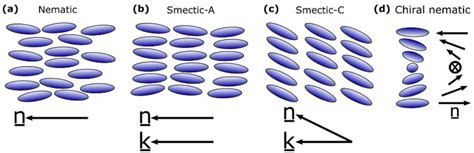
\includegraphics[width=.9\linewidth]{smecticCrystals.jpg}
\end{center}
\caption{\small Slika prikazuje, kako različne vrste smektičnih kristalov. Vir:\cite{daken_smectic_2022} }
\end{slika}

V smektikih A kaže odlikovana smer, ki ji pravimo direktor vzdolž normale plasti, v smektikih C* pa je kot, ki ga oklepa direktor z normalo nekje med \(10^{\circ} \text{ in } 30^{\circ}\).

Feroelektrične smektične C* tvorijo molekule, ki imajo velik električni dipolni moment prečno na vzdolžno os molekul, zato se v teh snoveh pojavi električna polarizacija, ki leži v ravnini plasti in je pravokotna na direktor. Polarizacija je sorazmerna s kotom nagiba. Tekoči kristali so posebej uporabni zaradi dvolomnosti, ki izhaja iz orientacijske urejenosti molekul, kjer je optična os vzporedna z direktorjem.

V dovolj debelem vzorcu oriše smer nagiba in s tem tudi električna polarizacija poln krog (nekaj sto do tisoč plasti). Polarizacijo plasti lahko uredimo v isto smer bodisi z zunanjim električnim poljem bodisi z ograditvijo vzorca v ploščici, ki predpisujeta orientacijo molekul. Predpisovanje orientacij molekul je doseženo s kemično ali mehansko obdelavo površin.

Če je razmik med ploščicama dovolj majhen (reda v \(\mu m\)), se direktor postavi v predpisani smeri po vsem vzorcu. V takem površinko stabiliziranem feroelektričnem tekočem kristalu so plasti kristala pravokotne na ploščici, električna polarizacija pa leži v ravnini ploščic.

Če postavimo ta tanko površinko stabiliziran feroelektrični kristal v zunanje električno polje \(\vec{E}\), ki je pravokoten na ploščici, se električna polarizacija vzorca deloma zasuče v smeri polje. Tudi direktor se deloma zasuče na stožcu smeri, ki ga določa nagib direktorja glede na normalo plasti. Zasuk električne polarizacije je sorazmeren z električnim poljem, posledično je sorazmeren tudi zasuk optične osi.

Linearnemu odzivu lomnega količnika na zunanje električno polje pravimo \emph{elektrooptični pojav}. Zasuk polarizacije je v izmeničnem polju odvisen tudi od frekvence. Pri previsoki frekvenci polarizacija ne more več slediti polju. Odvisnost spremembe polarizacije \(\partial P\) od frekvence opišemo z Debyjevim relaksacijskim modelom

\begin{equation}
\label{eq:1}
\partial P = \partial P_0 \frac{1}{1 + i \omega \tau}
\end{equation}

kjer je \(\tau\) relaksacijski čas odvisen od viskoznosti tekočega kristala in od debeline vzorca.

Kot zasuka optične osi, ki je sorazmeren s spremembo polarizacije, ima enako frekvenčno odvisnost.

Spremembo smeri optične osi zaznamo tako, da opazujemo, kako se spremeni polarizacija svetlobe pri prehodu skozi vzorec. Na vzorec posvetimo s polarizirano svetlobo in merimo svetlobno moč, ki jo prepušča analizator za vzorcem.

Vpadno polarizacijo razstavimo na izredno komponento, ki je vzporedna z optično osjo in na redno komponento, pravokotno na optično os. Prepuščeno svetlobno moč merimo s pomočjo fotodiode. Odziv nekega sistema na majhne periodične zunanje motnje najlažje izmerimos faznim občutljivim ojačevalnikom (FOO, angl. \emph{lock-in amplifier}).

FOO deluje po principu tega, da vhodni izmenični signal iz fotodiode pomnoži z referenčnim izmeničnim signalom s frekvenco modulacije (v našem primeru zunanje električnega polja, priklopljenega na tekočekristalni vzorec).

V tekočem kristalu je zasuk optične osi \(\psi\) zaradi viskoznosti snovi zakasnjen glede na zunanje električno polje. Del, ki je v fazi dobimo kot realni del enačbe \ref{eq:1}, del zasukan za \(\frac{\pi}{2}\) pa kot imaginarni del

\begin{align}\label{al:1}
  \psi_r &= \frac{\psi_0}{1 + (\omega \tau ) ^2} \\
\psi_i &= - \frac{\psi_0 \omega}{1 + (\omega \tau)^2}
\end{align}
\clearpage
\section{Potrebščine}\label{sec:orgb767dad}

\begin{itemize}
\item laser
\item FOO z multimetrom
\item fotodioda
\item analizator
\item vzorec
\item osciloskop
\end{itemize}
\section{Naloge}\label{sec:org943583a}

\begin{itemize}
\item prepričaj se, da je elektrooptični odziv sorazmeren z modulacijjo do neke napetosti
\item nariši obe komponentni signala kot funkciji frekvence in določi relaksacijski čas

\end{itemize}
\section{Izračuni}\label{sec:org6a1e141}
\subsection{Sorazmernost odziva z modulacijo}\label{sec:org3793a0c}

Pri fiksni frekvenci \(\nu = 20 \mathrm{Hz}\) sem preveril, če sta je realna komponenta signala odziva res sorazmerna. S prilagajanjem premice se vidi, da je odziv res linearen na \ref{slika:1}.

\begin{slika}[H]
\begin{center}
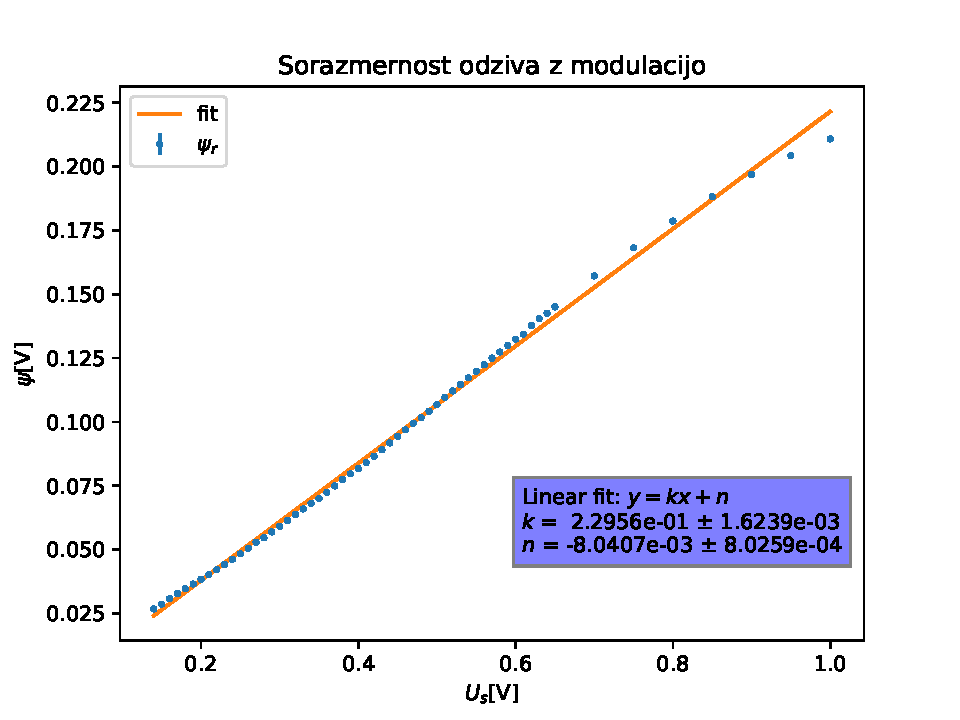
\includegraphics[width=.9\linewidth]{figures/modulacija.pdf}
\end{center}
\caption{\small Linearen odziv pri modulaciji je opazen. }\label{slika:1}
\end{slika}
\subsection{Določanje relaksacijskega časa}\label{sec:org628c203}

Sedaj sem pri fiksni napetosti \(U = 0.2 \mathrm{V}\) spreminjal frekvenco.

S prilagajanjem funkcij \ref{al:1} sem določil relaksacijski čas za vzorec

\[ \tau_1 = 2.98 \cdot 10^{-3} \pm 0.09 10^{-3} \mathrm{s} \quad \tau_2 = 2.10 \cdot 10^{-3} \pm 0.04 10^{-3} \mathrm{s}
\]

\begin{slika}[H]
  \begin{center}
    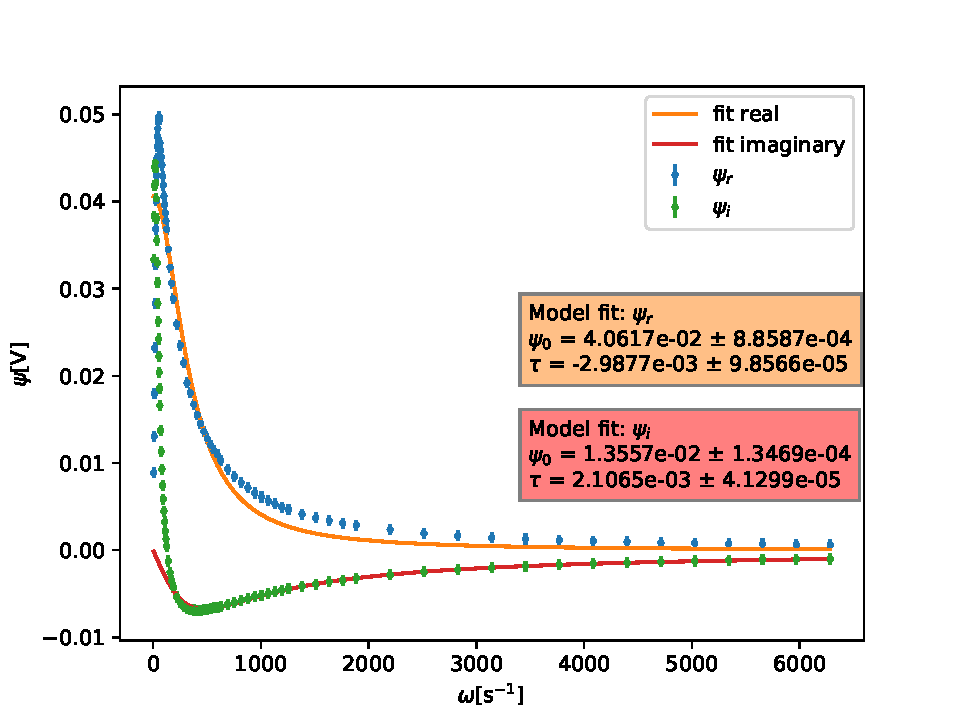
\includegraphics[width=.9\linewidth]{figures/fit_modelov}
  \end{center}
  \caption{\small Regresija modelov za \ref{al:1}}
\end{slika}


Za konec sem pa izračunal \(\tau\) še tako, da sem izračunal kvocient realne in imaginarne komponente. Z deljenjem \ref{al:1} dobimo

\[ \frac{\psi_i}{\psi_r} = - \tau \omega
\]

\begin{slika}[H]
  \begin{center}
    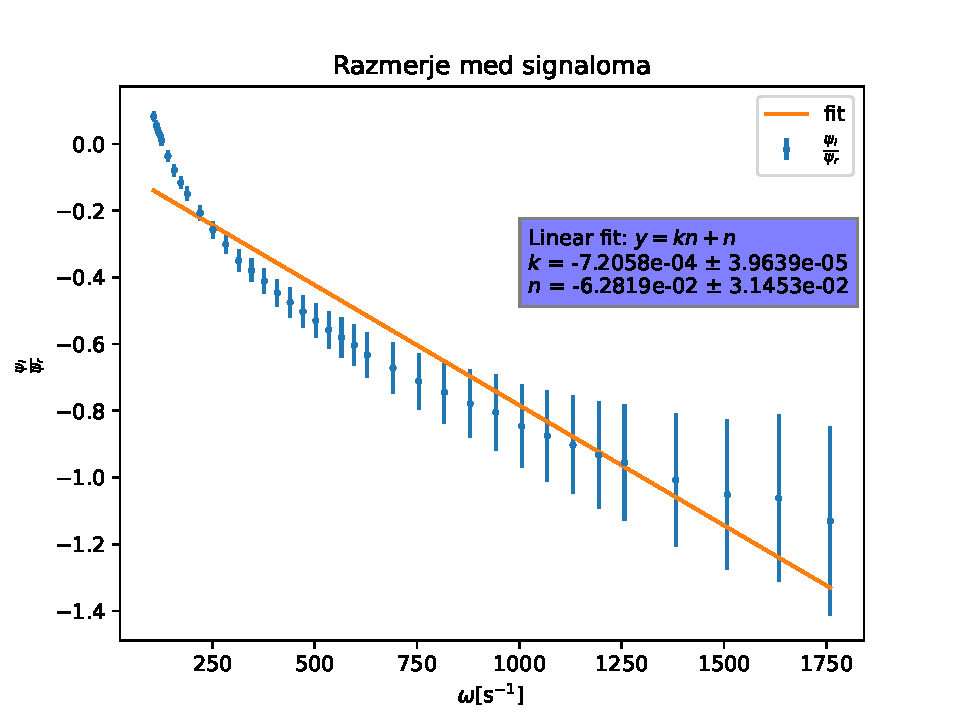
\includegraphics[width=.9\linewidth]{figures/deljena}
  \end{center}
  \caption{\small Zdeljena oblika, ki naj bi bila premica po krožni frekvenci \( \omega \) z naklonom \( \tau \). Napake hitro rastejo, saj je relativna npaka imaginarne komponente \( x \) velika.}
\end{slika}


Tako sem dobil še čas

\[ \tau = (0.72 \cdot 10^{-3} \pm 0.04) \mathrm{s}
\]

Kar pa se zelo slabo ujema s prej dobljenima časoma fittanja premic. Možno je, da je do napake prišlo zaradi nepoznavanja FOO in sem tekom merjenj nevede spremenil koeficient, s katerim je bil pomnožena izmerjena realna in imaginarna komponenta signala.


%\clearpage
%\addcontentsline{toc}{chapter}{Viri}
\bibliographystyle{plain}
\bibliography{refs.bib}
\end{document}
